\section{zadanie 6}
Zadanie polegało na skorzystaniu z wcześniej zaprogramowanej metod w celu znalezienia miejsc zerowych funkcji \[f_1(x) = e^{1-x} - 1\] oraz \[f_2(x) = x e^{-x}\]
Dokładność obliczeń będzie ograniczona przez \(\delta = 10^{-5}\) i \(\epsilon = 10^{-5}\).
Dokładne współrzędne x-owe miejsc zerowych dla funkcji to \(f_1(1) = 0\) i \(f_2(0) = 0\).
\begin{figure}[ht]
  \centering
  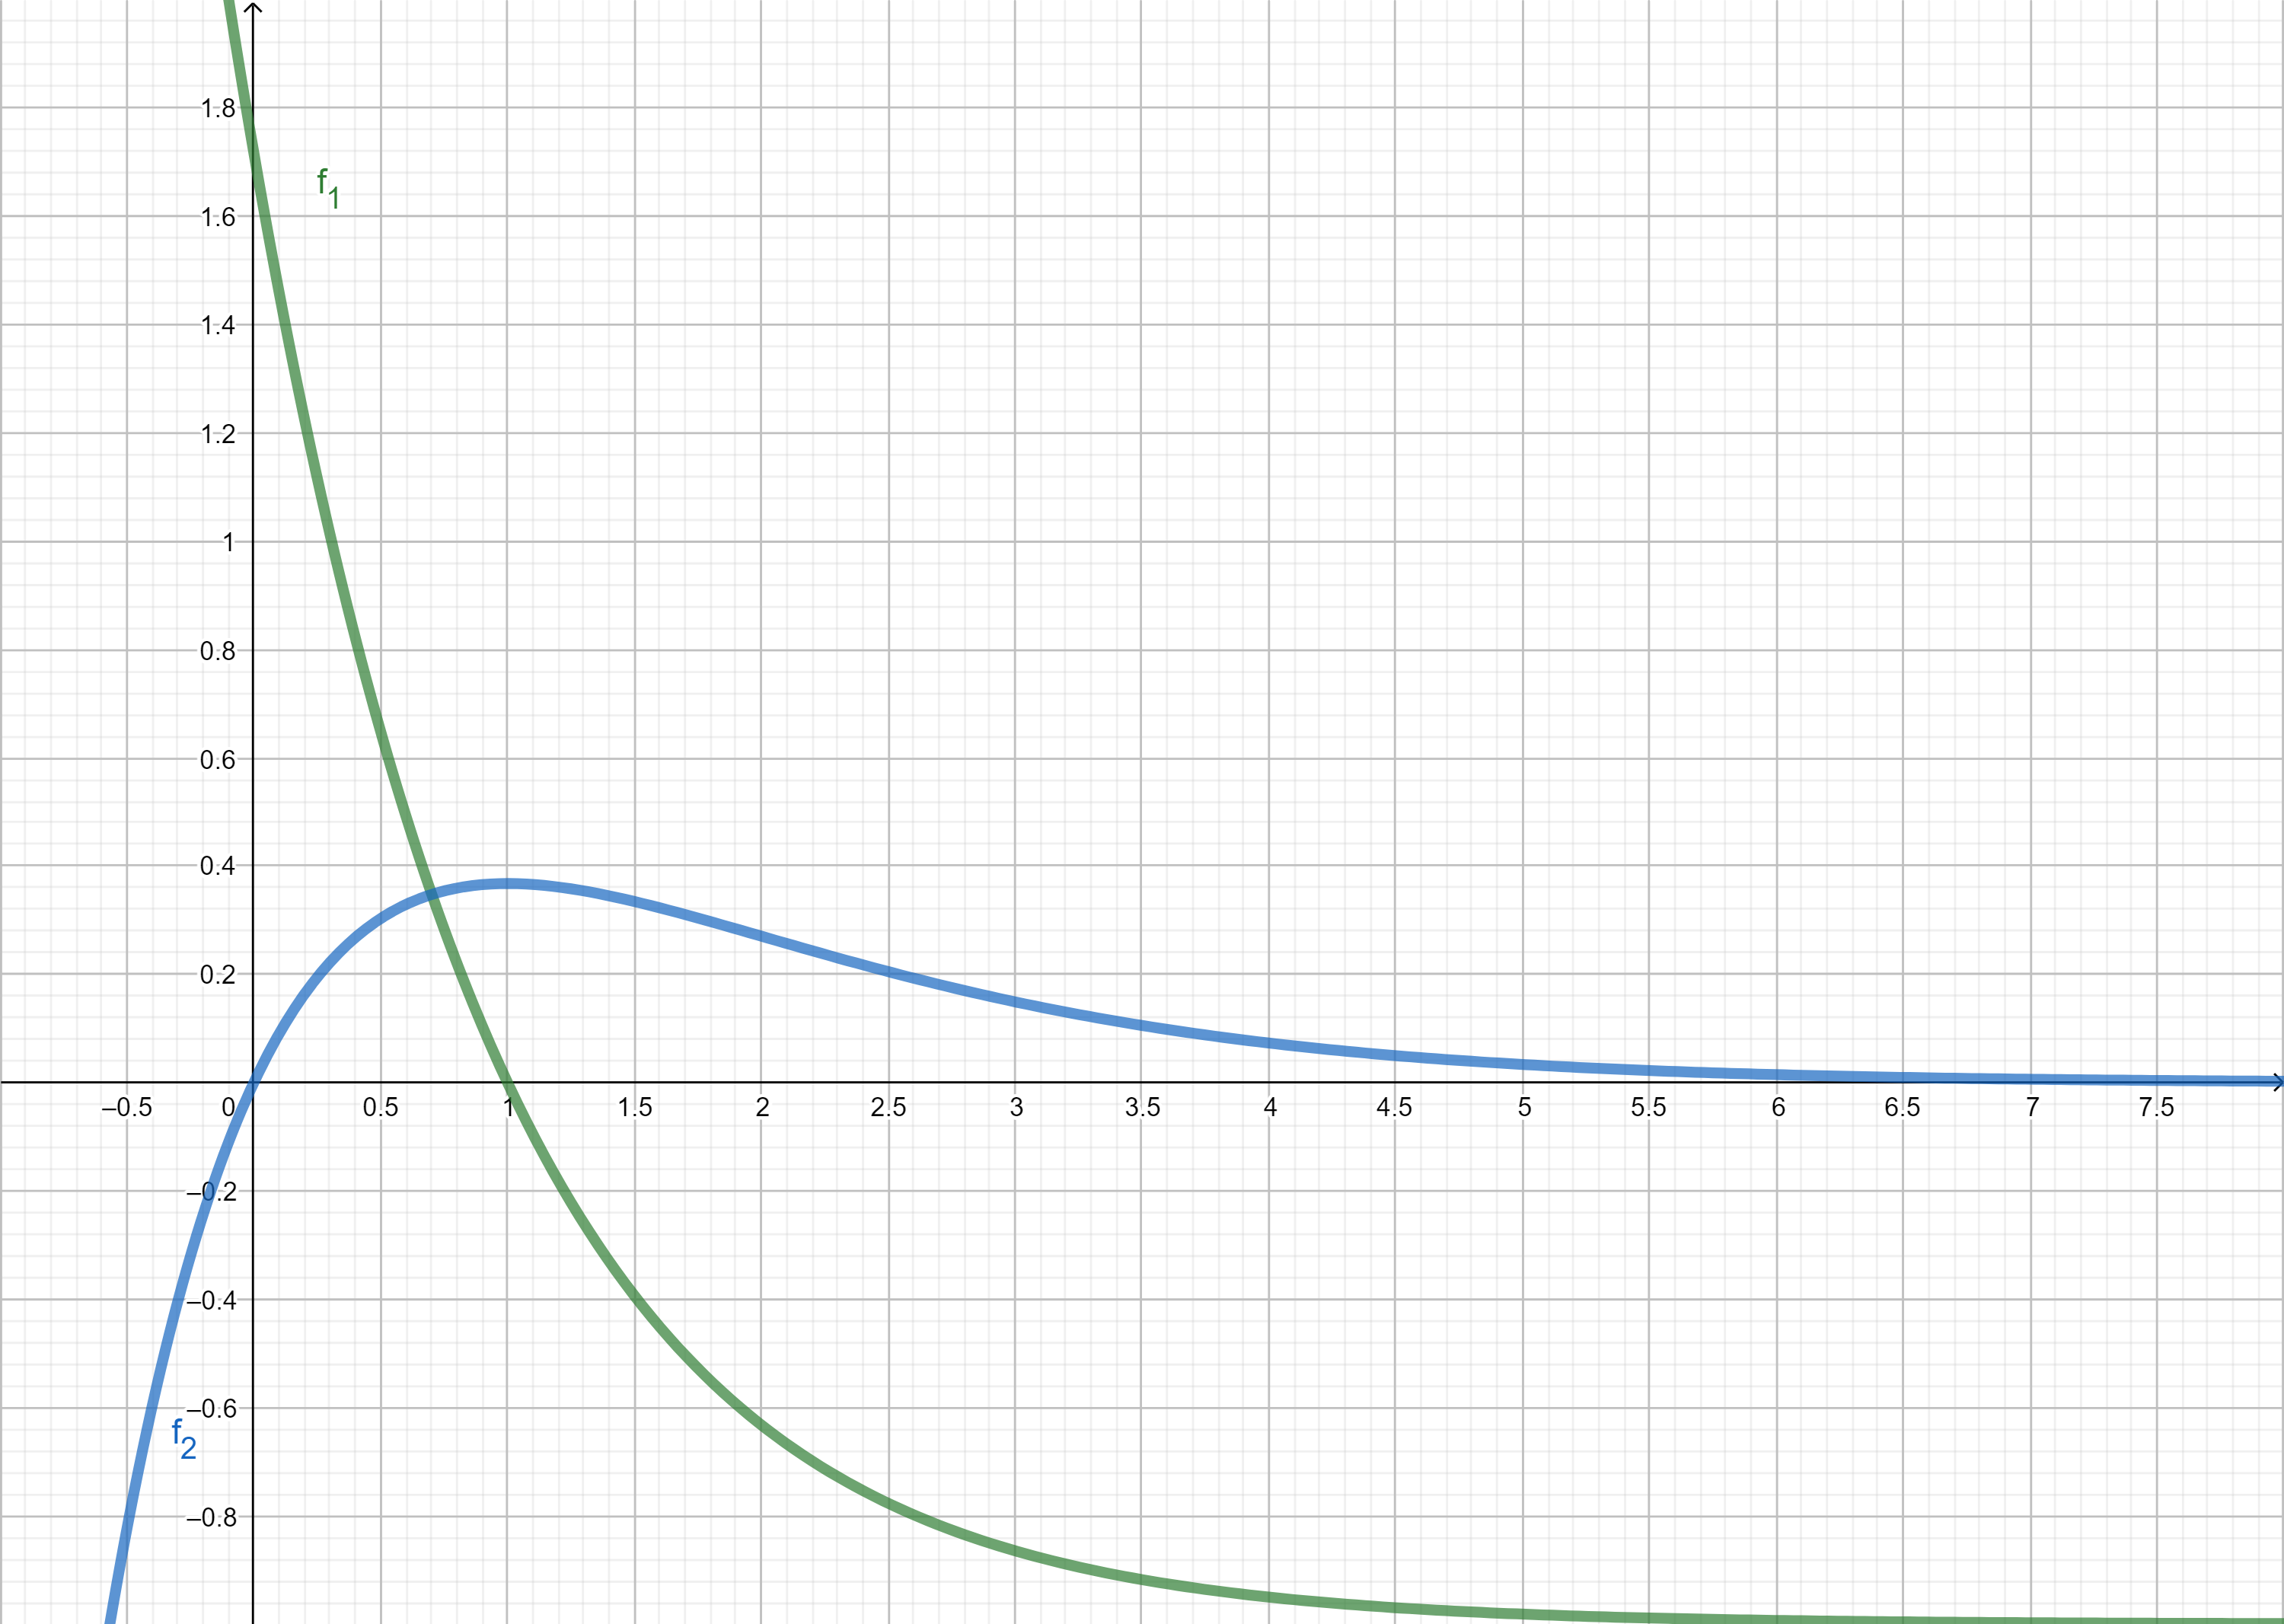
\includegraphics[width=\textwidth]{zadanie6.png}
  \caption{Wykresy funkcji \(f_1(x)\) oraz \(f_2(x)\)}
\end{figure}

\subsection{Wyniki:}
Wyniki działania programu znajdują się w poniższych tabelach
\begin{table}[ht]
  \makebox[\textwidth]{
    \centering
    \begin{tabular}{|c|c|c|c|c|}
    \hline
    przedział początkowy & funkcja & \(x\) & \(h(x)\) & iter \\
    \hline
    \hline
    \([0.5, 1.5]\) & \(f_1\) & 1.0 & 0.0 & 1 \\
    \([-5, 15]\) & \(f_1\) & 1.0000038146972656 & -3.814689989667386e-6 & 20 \\
    \([-15, 25]\) & \(f_1\) & 1.0000038146972656 & -3.814689989667386e-6 & 21 \\
    \([-0.5, 1.0]\) & \(f_2\) & -7.62939453125e-6 & -7.629452739132958e-6 & 16 \\
    \([-2, 15]\) & \(f_2\) & 1.9073486328125e-6 & 1.9073449948371624e-6 & 19 \\
    \([-1, 25]\) & \(f_2\) & 3.814697265625e-6 & 3.814682713737527e-6 & 19 \\
    \hline
    \end{tabular}
    }
    \caption{wartości z wyjścia programu \textbf{zadanie6.jl - metoda bisekcji}}
\end{table}

Przedział którego środkiem będzie miejsce zerowe to w metodzie bisekcji dokładny i natychmiastowy wynik nie zależnie od długości przedziału. Zwiększenie długości przedziału oraz przesunięcie jego środka ma wpływ na ilość wykonywanych iteracji;

\begin{table}[ht]
  \makebox[\textwidth]{
    \centering
    \begin{tabular}{|c|c|c|c|c|}
    \hline
    przedział początkowy & funkcja & \(x\) & \(h(x)\) & iter \\
    \hline
    \hline
    \(1.0\) & \(f_1\) & 1.0 & 0.0 & 1 \\
    \(1.5\) & \(f_1\) & 0.9999999984736215 & 1.5263785790864404e-9 & 4 \\
    \(2.5\) & \(f_1\) & 0.9999934982589662 & 6.501762170207925e-6 & 6 \\
    \(0.1\) & \(f_2\) & -1.4906619716777104e-8 & -1.490661993898442e-8 & 3 \\
    \(0.5\) & \(f_2\) & -3.0642493416461764e-7 & -3.0642502806087233e-7 & 5 \\
    \(1.1\) & \(f_2\) & 14.272123938290509 & 9.040322779745447e-6 & 3 \\
    \hline
    \end{tabular}
    }
    \caption{wartości z wyjścia programu \textbf{zadanie6.jl - metoda stycznych}}
\end{table}

Metoda Newtona radzi sobie szybciej ze znalezieniem miejsc zerowych ale przez fakt że używamy pochodnych do "przewidywania" gdzie miejsce zerowe może leżeć, ta metoda nie zawsze odnajdzie prawdziwe miejsce zerowe. Przykładem tego może być ostatni wynik w tabeli dla funkcji \(f_2\), \((\lim_{x \to \infty}{f_2} = 0)\) gdzie dla punktu startowego \(x_0 = 1.1\) tuż "za" ekstremum funkcji metoda "znalazła" przybliżenie miejsca zerowego mimo że go tam nie ma.

\begin{table}[ht]
  \makebox[\textwidth]{
    \centering
    \begin{tabular}{|c|c|c|c|c|}
    \hline
    przedział początkowy & funkcja & \(x\) & \(h(x)\) & iter \\
    \hline
    \hline
    \([0.5 , -1.0]\) & \(f_1\) & 0.9999977863660099 & 2.2136364401514896e-6 & 5 \\
    \([-5.0 , 5.0]\) & \(f_1\) & 4.975665372740593 & -0.9812331895845449 & 3 \\
    \([-5.0 , 25.0]\) & \(f_1\) & 24.92563743470281 & -0.9999999999593343 & 3 \\
    \([-1.0 , 0.5]\) & \(f_2\) & -1.1737426154042664e-6 & -1.1737439930768023e-6 & 7 \\
    \([-5.0 , 5.0]\) & \(f_2\) & 14.70482129398244 & 6.04278309521908e-6 & 13 \\
    \([-5.0 , 25.0]\) & \(f_2\) & 24.999999999985963 & 3.471985966287791e-10 & 1 \\
    \hline
    \end{tabular}
    }
    \caption{wartości z wyjścia programu \textbf{zadanie6.jl - metoda siecznych}}
\end{table}

W metodzie siecznych podobnie jak w metodzie stycznych źle dobrane wartości początkowe mogą dać niepoprawne wyniki. Widać również że przez zbyt długi przedział metoda może zwrócić błędne wyniki.
\subsection{b)}
Co się stanie, gdy w metodzie Newtona dla \(f_1\) wybierzemy \(x_0 \in (1, \infty]\) a dla \(f_2\) wybierzemy \(x_0 > 1\), oraz \(x_0 = 1\) dla \(f_2\)?

\begin{table}[ht]
  \makebox[\textwidth]{
    \centering
    \begin{tabular}{|c|c|c|c|c|c|}
    \hline
    \(x_0\) & funkcja & \(x\) & \(h(x)\) & iter & error \\
    \hline
    \hline
    \(1.0\) & \(f_1\) & 0.9999999810061002 & 1.8993900008368314e-8 & 5 & 0\\
    \(1.5\) & \(f_1\) & 0.9999999995278234 & 4.721767421500545e-10 & 21 & 0 \\
    \(2.5\) & \(f_1\) & nothing & nothing & nothing & 1 \\
    \(0.1\) & \(f_2\) & 14.398662765680003 & 8.03641534421721e-6 & 10 & 0 \\
    \(0.5\) & \(f_2\) & 14.398662765680003 & 8.03641534421721e-6 & 9 & 0 \\
    \(1.1\) & \(f_2\) & 14.636807965014 & 6.438155219843286e-6 & 6 & 0 \\
    \(1.1\) & \(f_2\) & nothing & nothing & nothing & 2 \\
    \hline
    \end{tabular}
    }
    \caption{wartości z wyjścia programu \textbf{zadanie6.jl}}

\end{table}

\subsection{Wnioski:}
Dla \(f_1\) wybierając punkt początkowy \(x_0 \in (1, \infty]\) pochodna \(x \to \infty\) dąży do 0, przez co dla \(x_0 = 8.0\) metoda zwracała błąd o przekroczeniu maksymalnej liczny iteracji.
Dla \(f_2\) wybierając punkt początkowy \(x_0 \in (1, \infty]\) tak jak w ostatnim przypadku dla tej metody pochodna będzie przybliżać miejsce zerowe którego tam tak naprawdę nie ma. Wybierając \(x_0 = 1.0\) wartość pochodnej w tym punkcie wynosi 0 zatem metoda zwraca błąd "2" mowiący o wartości pochodnej bliskiej 0.